\documentclass[tikz,border=8pt]{standalone}
\usepackage{amsmath}
\usetikzlibrary{arrows.meta,positioning,calc,fit}

\begin{document}
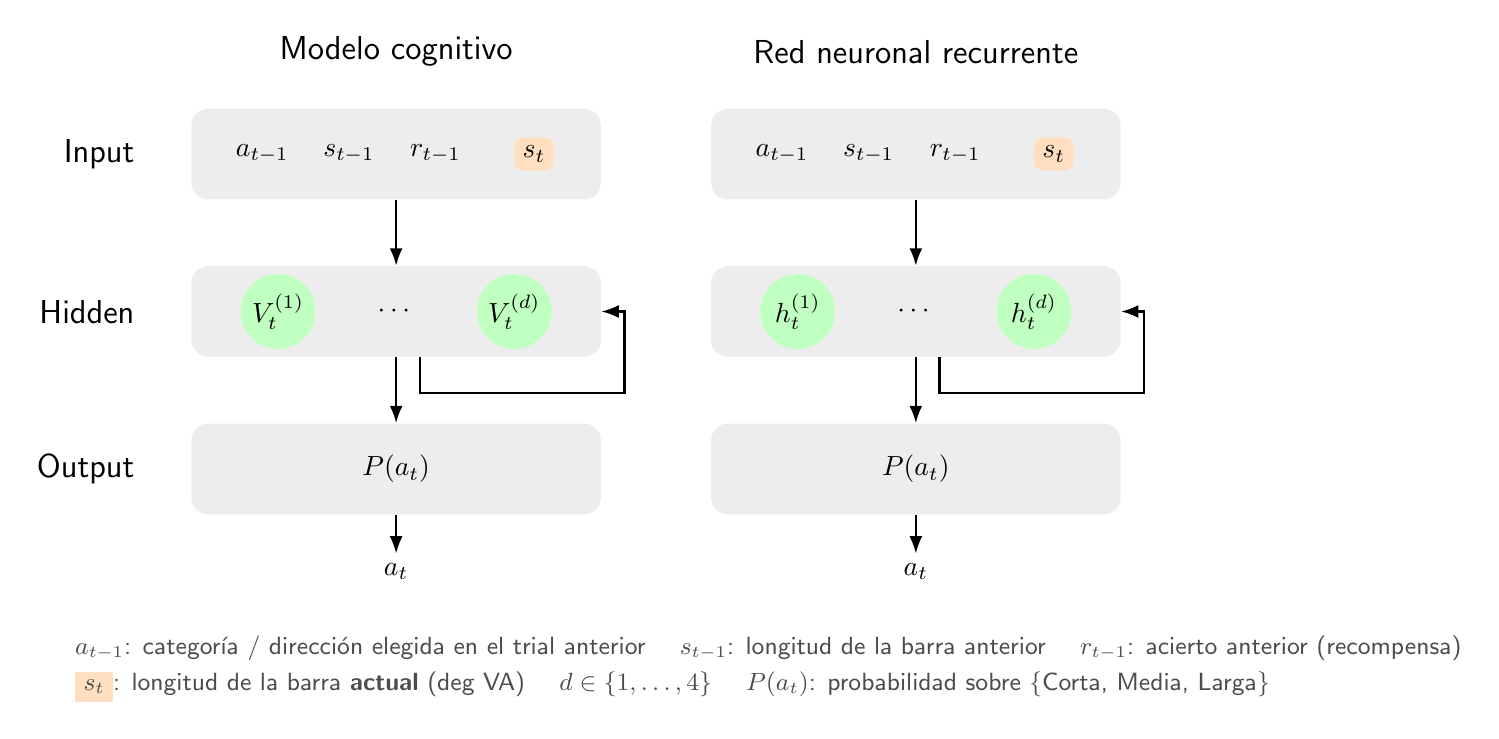
\begin{tikzpicture}[
  font=\sffamily,
  band/.style={rounded corners=6pt, fill=black!7, draw=none, inner sep=8pt, minimum height=1.15cm},
  unit/.style={circle, fill=green!25, draw=none, minimum size=0.95cm, inner sep=0pt},
  flow/.style={-{Latex[length=2.2mm]}, line width=0.8pt},
  rowlab/.style={anchor=east, font=\sffamily\large},
  now/.style={fill=orange!25},
]

% ---------- row labels (shared) ----------
\node[rowlab] (Lin)  at (-0.6, 0)    {Input};
\node[rowlab] (Lhid) at (-0.6,-2.0)  {Hidden};
\node[rowlab] (Lout) at (-0.6,-4.0)  {Output};

% ================= LEFT: cognitive model =================
\begin{scope}[xshift=0cm]
  \node[font=\sffamily\large] at (2.6, 1.3) {Modelo cognitivo};

  % input band
  \node[band, minimum width=5.2cm] (Lband_in) at (2.6,0) {};
  \node at (0.9,0) {$a_{t-1}$};
  \node at (2.0,0) {$s_{t-1}$};
  \node at (3.1,0) {$r_{t-1}$};
  \node[now, rounded corners=3pt, inner sep=3pt] at (4.35,0) {$s_{t}$};

  % hidden band
  \node[band, minimum width=5.2cm] (Lband_h) at (2.6,-2.0) {};
  \node[unit] (LV1) at (1.1,-2.0) {$V_t^{(1)}$};
  \node at (2.6,-2.0) {$\cdots$};
  \node[unit] (LVd) at (4.1,-2.0) {$V_t^{(d)}$};

  % output band
  \node[band, minimum width=5.2cm] (Lband_out) at (2.6,-4.0) {$P(a_t)$};
  \node (La) at (2.6,-5.3) {$a_t$};

  \draw[flow] (Lband_in.south) -- (Lband_h.north);
  \draw[flow] (Lband_h.south) -- (Lband_out.north);
  \draw[flow] (Lband_out.south) -- (La);
  % recurrence
  \draw[flow] (Lband_h.south) ++(0.3,0) |- ++(2.6,-0.45) |- ($(Lband_h.east)+(0,0)$);
\end{scope}

% ================= RIGHT: recurrent neural network =================
\begin{scope}[xshift=6.6cm]
  \node[font=\sffamily\large] at (2.6, 1.3) {Red neuronal recurrente};

  \node[band, minimum width=5.2cm] (Rband_in) at (2.6,0) {};
  \node at (0.9,0) {$a_{t-1}$};
  \node at (2.0,0) {$s_{t-1}$};
  \node at (3.1,0) {$r_{t-1}$};
  \node[now, rounded corners=3pt, inner sep=3pt] at (4.35,0) {$s_{t}$};

  \node[band, minimum width=5.2cm] (Rband_h) at (2.6,-2.0) {};
  \node[unit] (Rh1) at (1.1,-2.0) {$h_t^{(1)}$};
  \node at (2.6,-2.0) {$\cdots$};
  \node[unit] (Rhd) at (4.1,-2.0) {$h_t^{(d)}$};

  \node[band, minimum width=5.2cm] (Rband_out) at (2.6,-4.0) {$P(a_t)$};
  \node (Ra) at (2.6,-5.3) {$a_t$};

  \draw[flow] (Rband_in.south) -- (Rband_h.north);
  \draw[flow] (Rband_h.south) -- (Rband_out.north);
  \draw[flow] (Rband_out.south) -- (Ra);
  \draw[flow] (Rband_h.south) ++(0.3,0) |- ++(2.6,-0.45) |- (Rband_h.east);
\end{scope}

% ---------- legend for CenterTask ----------
\node[align=left, anchor=north west, font=\sffamily\small, text=black!70] at (-1.6,-6.0) {%
  $a_{t-1}$: categoría / dirección elegida en el trial anterior \quad
  $s_{t-1}$: longitud de la barra anterior \quad
  $r_{t-1}$: acierto anterior (recompensa)\\[2pt]
  \colorbox{orange!25}{$s_t$}: longitud de la barra \textbf{actual} (deg VA) \quad
  $d \in \{1,\dots,4\}$ \quad
  $P(a_t)$: probabilidad sobre \{Corta, Media, Larga\}
};
\end{tikzpicture}
\end{document}
